\chapter{The SABR model}
\label{cap:sabr}

Heston describes the \emph{whole} surface with five parameters. SABR (Hagan, Kumar, Lesniewski and Woodward, 2002)
makes a different choice: it describes \emph{one smile at a time} (one expiry) with three nearly independent
parameters and, above all, it provides an \textbf{approximate implied volatility formula} that is computed
instantly. It is the market standard in interest rates and is also useful in equities for interpolating smiles.

Hagan's formula, however, is an \emph{asymptotic expansion}, not the model. This chapter derives the formula,
checks it against two Monte Carlo simulations of the true model, and measures where it stops being valid.

\section{The dynamics}
\begin{equation}\label{eq:sabr}
\dd F_t=\alpha_tF_t^\beta\dd W_t,\qquad\dd\alpha_t=\nu\,\alpha_t\dd Z_t,\qquad\dd\langle W,Z\rangle_t=\rho\dd t .
\end{equation}
Here $\alpha_t$ is a lognormal stochastic volatility without mean reversion, with initial value $\alpha$; $\nu\ge0$ is
its volatility (vol-of-vol), per $\sqrt{\text{year}}$; $\rho$ is the correlation between forward and volatility;
$\beta\in[0,1]$ is the ``elasticity exponent''.

\subsection{\texorpdfstring{Why $\beta=1$ for the SPX}{Why β=1 for the SPX}}
\begin{perche}
\begin{itemize}
\item \textbf{$\beta$ is not identifiable from a smile.} Both $\beta$ and $\rho$ produce slope: the ATM slope is
about $-\tfrac12(1-\beta)\sigma_{\mathrm{ATM}}+\tfrac12\rho\nu$. Moreover, the level
$\sigma_{\mathrm{ATM}}\approx\alpha F^{\beta-1}$ makes $\alpha$ trade off against $\beta$. With $\beta$ free the
$(\alpha,\beta,\rho)$ calibration is ill-conditioned; Hagan et al.\ themselves write that estimating $\beta$ from the
smile amounts to ``fitting the noise''.
\item \textbf{$\beta$ is a choice of dynamics, not of price.} It decides how the ATM volatility moves when the forward
moves (the \emph{backbone}): it changes the deltas, not today's prices.
\item \textbf{$\beta=1$ is natural for an equity index.} The model is lognormal and \emph{scale-free}: the volatility
depends only on $K/F$, $\alpha$ is directly a volatility, and all the price--volatility co-movement sits in $\rho$.
\item \textbf{It is numerically convenient.} No boundary at $F=0$, positive and martingale simulation, ATM inversion
via a quadratic equation.
\end{itemize}
\end{perche}

With $\beta=1$, by Itô and the explicit solution of geometric Brownian motion:
\begin{equation}\label{eq:sabr-beta1}
\dd\ln F_t=-\tfrac12\alpha_t^2\dd t+\alpha_t\dd W_t,\qquad \alpha_t=\alpha\,e^{\nu Z_t-\nu^2t/2}\quad\text{(exact)}.
\end{equation}

\subsection{Model facts that matter}
For $\beta=1$ two results of Lions and Musiela (2007) hold.
\begin{itemize}
\item \textbf{Martingale.} $F$ is a true martingale if and only if $\rho\le0$. For $\rho>0$ it is a strict local
martingale: $\E F_T<F$.
\item \textbf{Moments.} For $m>1$, $\E F_T^m<\infty$ if and only if $\rho\le-\sqrt{(m-1)/m}$. In particular
$\Var F_T<\infty$ only if $\rho\le-1/\sqrt2\approx-0.71$. At $\rho=0$ all moments of order $>1$ are infinite.
\end{itemize}
\begin{attenzione}
Practical consequence: the call payoff can have infinite variance, so the standard error of an MC estimate on calls is
not reliable. We simulate \textbf{puts} (payoff bounded by $K$). Calls are obtained by parity with $F$, but only for
$\rho\le0$ (Section~\ref{sec:sabr-rho-pos}).
\end{attenzione}

\section{\texorpdfstring{Hagan's formula ($\beta=1$)}{Hagan's formula (β=1)}}
With $k=\ln(K/F)$:
\begin{equation}\label{eq:hagan}
\boxed{\sigma_H(K)=\alpha\,\frac{z}{x(z)}\,\big(1+c_1T\big)},\qquad z=\frac\nu\alpha\ln\frac FK=-\frac{\nu k}{\alpha},\qquad
c_1=\frac{\rho\nu\alpha}4+\frac{2-3\rho^2}{24}\nu^2,
\end{equation}
\begin{equation}\label{eq:hagan-x}
x(z)=\ln\frac{D(z)+z-\rho}{1-\rho}=\int_0^z\frac{\dd u}{D(u)},\qquad D(z)=\sqrt{1-2\rho z+z^2}.
\end{equation}
The price is obtained by plugging $\sigma_H(K)$ into the Black formula \eqref{eq:black}:
\[
V=\mathrm{Black}\big(F,K,T,\DF,\sigma_H(K)\big).
\]

\subsection{\texorpdfstring{Where the factor $z/x(z)$ comes from}{Where the factor z/x(z) comes from}}
\noindent\textbf{Step 1.} Measure the distance to the strike in units of the current volatility:
$u_t=\ln(F_t/K)/\alpha_t$.

\noindent\textbf{Step 2.} By Itô, neglecting the $\dd t$ terms, $\dd u=\dd W-\nu u\,\dd Z$. Its ``diffusion speed''
is
\[
\frac{\dd\langle u\rangle}{\dd t}=1-2\rho\nu u+\nu^2u^2=D(\nu u)^2 .
\]
This is the only place where $\rho$ and $\nu$ enter at leading order.

\noindent\textbf{Step 3.} For short times the probability of reaching the strike decays like $e^{-\delta^2/2T}$,
where $\delta$ is the distance measured with this variable speed:
\[
\delta=\int_0^{u_0}\frac{\dd u}{D(\nu u)}=\frac{x(z)}{\nu},\qquad z=\nu u_0 .
\]
\noindent\textbf{Step 4.} In Black with volatility $\sigma$ the same distance is $\ln(F/K)/\sigma$. Equating the two
distances:
\[
\sigma=\frac{\nu\ln(F/K)}{x(z)}=\alpha\,\frac{z}{x(z)} .
\]
As $K\to F$ we have $z/x\to1$.

\begin{idea}
The implied volatility at a strike is, approximately, the volatility ``seen'' along the most likely path to that
strike. With $\rho<0$, moving down towards low strikes means that volatility rises: hence the skew. The vol-of-vol
makes both wings expensive, because large moves happen in high-volatility states.
\end{idea}

\subsection{\texorpdfstring{The factor $(1+c_1T)$: a check at $\rho=0$}{The factor (1+c₁T): a check at ρ=0}}
The factor $(1+c_1T)$ is the first correction in $T$; its full derivation is in the appendix of Hagan et al. The
$\rho=0$ part, however, can be checked by hand.

\noindent\textbf{Step 1.} At $\rho=0$, given the path of $\alpha$, $\ln F_T$ is Gaussian with variance
$I=\int_0^T\alpha_t^2\dd t$. The price is the average of Black prices, and ATM Black is linear in $\sqrt I$ at first
order. Hence $\sigma_{\mathrm{ATM}}\approx\E\sqrt{I/T}$.

\noindent\textbf{Step 2.} Write $I/(\alpha^2T)=1+\epsilon$ with $\E\epsilon=\nu^2T/2+O(\nu^3)$ and
$\E\epsilon^2=4\nu^2T/3+O(\nu^3)$ (from the expansion of $e^{2\nu Z_t-\nu^2t}$ and the moments of Brownian motion).

\noindent\textbf{Step 3.} With $\sqrt{1+\epsilon}\approx1+\tfrac12\epsilon-\tfrac18\epsilon^2$:
\[
\E\sqrt{1+\epsilon}\approx1+\frac{\nu^2T}{4}-\frac{\nu^2T}{6}=1+\frac{2\nu^2T}{24},
\]
which is exactly $c_1T$ at $\rho=0$.

\subsection{Near the money: three nearly orthogonal knobs}
Expanding for small $k$:
\begin{equation}\label{eq:sabr-taylor}
\sigma_H\approx(1+c_1T)\Big[\alpha+\tfrac12\rho\nu\,k+\frac{(2-3\rho^2)\nu^2}{12\alpha}k^2\Big].
\end{equation}
\begin{itemize}
\item $\alpha$ sets the \textbf{level};
\item $\rho\nu$ sets the \textbf{slope}: ATM skew $=\tfrac12\rho\nu(1+c_1T)$;
\item $\nu^2/\alpha$ sets the \textbf{curvature}.
\end{itemize}
This also gives good starting values for the calibration: fit a parabola $\sigma_0+Sk+\tfrac12Ck^2$ to the
near-the-money data and invert the relations.

\section{\texorpdfstring{The ATM inversion for $\alpha$}{The ATM inversion for α}}
\subsection{The quadratic equation}
As $K\to F$, $\sigma_{\mathrm{ATM}}=\alpha(1+c_1T)$. Substituting $c_1$:
\[
\sigma_{\mathrm{ATM}}=\alpha\Big(1+\frac{(2-3\rho^2)\nu^2T}{24}\Big)+\alpha^2\,\frac{\rho\nu T}{4}.
\]
Given the market $\sigma_{\mathrm{ATM}}$, $\alpha$ therefore solves
\begin{equation}\label{eq:alpha-atm}
a\alpha^2+b\alpha-\sigma_{\mathrm{ATM}}=0,\qquad a=\frac{\rho\nu T}{4},\qquad b=1+\frac{(2-3\rho^2)\nu^2T}{24}.
\end{equation}
With $\beta<1$ it would be a cubic equation; $\beta=1$ removes the $\alpha^3$ term.

\subsection{Which root, and in what form}
The textbook formula $(-b+\sqrt{b^2+4a\sigma_{\mathrm{ATM}}})/(2a)$ suffers cancellation as $a\to0$ (that is,
$\rho\nu\to0$). Rationalizing gives the stable form
\begin{equation}\label{eq:alpha-stabile}
\alpha=\frac{2\sigma_{\mathrm{ATM}}}{b+\sqrt{b^2+4a\sigma_{\mathrm{ATM}}}},
\end{equation}
which tends to $\sigma_{\mathrm{ATM}}/b$ as $a\to0$ with no division by zero.

It is the \emph{small} root, the one for which the correction $(1+c_1T)$ stays $\ge b/2$. On the other root the
``correction'' would dominate the leading term, and the expansion would make no sense. For $\rho>0$ the product of
the roots is $-\sigma_{\mathrm{ATM}}/a<0$: there is exactly one positive root.

\subsection{\texorpdfstring{The feasibility ceiling for $\rho<0$}{The feasibility ceiling for ρ<0}}
For $\rho<0$ we have $a<0$, and the function $\alpha\mapsto\sigma_{\mathrm{ATM}}(\alpha)=\alpha(b+a\alpha)$ is a
downward-opening parabola. It has a maximum at the vertex $\alpha^*=b/(2|a|)$, where it equals
\begin{equation}\label{eq:tetto}
\sigma_{\mathrm{ATM}}^{\max}=\frac{b^2}{4|a|}.
\end{equation}
Above this ceiling the discriminant is negative: \emph{no} $\alpha$ reproduces the given ATM volatility.

\begin{esempio}[title={Example: the ceiling at $\rho=-0.9$, $\nu=2$, $T=5$}]
\begin{itemize}
\item $a=\rho\nu T/4=-0.9\cdot2\cdot5/4=-2.25$.
\item $b=1+(2-3\cdot0.81)\cdot4\cdot5/24=1-0.43\cdot20/24\approx0.642$.
\item $\sigma_{\mathrm{ATM}}^{\max}=b^2/(4|a|)\approx0.412/9\approx0.0457$.
\end{itemize}
With these $(\rho,\nu)$ no ATM volatility above 4.57\% is attainable. At $\rho=-0.9$, $\nu=5$, $T=2$ the ceiling drops
to about 0.12\%, and these parameters lie within the plausible bounds of a calibration.
\end{esempio}

\begin{progetto}[title={In the qpricer project: ATM inversion}]
\code{alpha\_from\_atm} in \code{src/qpricer/models/sabr.py} uses \eqref{eq:alpha-stabile}. Above the ceiling it
returns \code{NaN} with a warning, never a clipped value. An independent check confirmed that this happens exactly
when no positive root exists (20{,}000 points), and that the root agrees with a numerical search on $[0,\alpha^*]$ to
within $10^{-13}$. The round trip $\sigma_{\mathrm{ATM}}(\hat\alpha)=\sigma_{\mathrm{ATM}}$ is exact to
$4.4\times10^{-16}$ wherever $b>0$, that is, for every $\rho\le0$.

\smallskip
In calibration (Chapter~\ref{cap:calibrazione}) the objective function uses $(\alpha,\rho,\nu)$ directly, and
\eqref{eq:alpha-stabile} serves only to build the starting points. Points without a positive root are discarded and
counted: 0 out of 195 across the 39 expiries.
\end{progetto}

\section{Evaluating the formula without losing digits}
\subsection{\texorpdfstring{The limit $z\to0$}{The limit z→0}}
For $K=F$ or $\nu=0$ we have $z=0$ and $z/x(z)$ is $0/0$. For $|z|<z_c=10^{-3}$ the series expansion is used:
\begin{equation}\label{eq:zx-serie}
\frac z{x(z)}=1-\frac{\rho z}2+\frac{(2-3\rho^2)z^2}{12}+\frac{\rho(5-6\rho^2)z^3}{24}+O(z^4).
\end{equation}
It is obtained by integrating the generating function of the Legendre polynomials, $1/D(u)=\sum_nP_n(\rho)u^n$, and
inverting the series. The coefficient of $z^4$ is at most 0.05 in absolute value, so at $z_c$ the series error is
$\le5\times10^{-14}$.

\subsection{Branching on sign, and \code{log1p}}
For $|z|\ge z_c$ we use \eqref{eq:hagan-x}, with two precautions.

\noindent\textbf{Step 1: no cancellation as $\rho\to\pm1$.} Write $D^2=(z-\rho)^2+(1-\rho)(1+\rho)$, a sum of
non-negative terms. For $z<\rho$ and $\rho$ close to $\pm1$ we have $D\approx\rho-z$, and $D+z-\rho$ cancels; we then
use the identity $(D+z-\rho)(D-z+\rho)=1-\rho^2$, which gives
\[
x(z)=\ln\frac{1+\rho}{D+\rho-z}\qquad(z<\rho).
\]
\noindent\textbf{Step 2: no loss of digits for small $z$.} For small $z$ the argument of the logarithm is $1+O(z)$,
and the direct logarithm has a relative error of about $4\varepsilon/|z|$ (with $\varepsilon=2^{-52}$). Instead,
``argument minus 1'' is computed exactly with the identity
\[
D-1=\frac{D^2-1}{D+1}=\frac{z(z-2\rho)}{D+1},
\]
and passed to \code{log1p}:
\begin{align*}
x&=\mathrm{log1p}\Big(\frac{z\,(D+1+z-2\rho)}{(D+1)(1-\rho)}\Big) &&\text{for } z\ge\rho,\\
x&=-\mathrm{log1p}\Big(-\frac{z\,(D+1+2\rho-z)}{(D+1)(1+\rho)}\Big) &&\text{for } z<\rho.
\end{align*}
The relative error is now $O(\varepsilon)$ for every $z$.

\subsection{Non-positive volatility}
If $c_1<0$ (for example with $|\rho|>\sqrt{2/3}$), for $T\ge1/|c_1|$ the factor $1+c_1T$ is $\le0$ and the formula
returns a non-positive volatility. The code returns \code{NaN} with a warning; it never clips.

\begin{progetto}[title={In the qpricer project: checks of the formula}]
\code{z\_over\_x} and \code{implied\_vol} in \code{src/qpricer/models/sabr.py}.
\begin{itemize}
\item Against a transcription of Hagan in 60-digit decimal arithmetic, on 1500 random points ($\alpha,\nu\le5$,
$|\rho|\le0.999$, $T\le30$, $|k|\le3$): relative error $5.0\times10^{-14}$.
\item Jump across $|z|=z_c$, net of the true slope: $4.7\times10^{-14}$ relative.
\item Symmetry at $\rho=0$, $\sigma(k)=\sigma(-k)$: $4.4\times10^{-16}$.
\item $x(z)$ against quadrature of $\int_0^z\dd u/D(u)$, including at $\rho=\pm0.999$: $2.9\times10^{-15}$.
\item Limit $\nu\to0$ (gate, threshold $10^{-10}$, $|k|\le1$, $T$ from 0.01 to 10, six values of $\rho$): at $\nu=0$
the gap from $\alpha$ is exactly 0; at $\nu=10^{-12}$ it is $3.0\times10^{-12}$.
\end{itemize}
\end{progetto}

\section{\texorpdfstring{SABR Monte Carlo ($\beta=1$)}{SABR Monte Carlo (β=1)}}
\subsection{Log-Euler with exact volatility}
On a grid $t_n=n\Delta$, with $Z_F=\rho Z_\alpha+\sqrt{1-\rho^2}Z_\perp$:
\begin{align}
\alpha_{n+1}&=\alpha_n\exp\big(\nu\sqrt\Delta Z_{\alpha,n}-\tfrac12\nu^2\Delta\big),\label{eq:sabr-alpha}\\
\ln F_{n+1}&=\ln F_n-\tfrac12\alpha_n^2\Delta+\alpha_n\sqrt\Delta\, Z_{F,n}.\label{eq:sabr-euler}
\end{align}
Properties:
\begin{itemize}
\item $\hat\alpha$ is exact in law on the grid ($\ln\alpha$ is a Brownian motion with drift);
\item $\hat F>0$ always;
\item $\E[\hat F_{n+1}\mid\mathcal F_{t_n}]=\hat F_n$ exactly, for every $\Delta$ and every $\rho$, by the same
argument used for Euler in Heston (Chapter~\ref{cap:mc}).
\end{itemize}
The only error comes from the integrated variance $I=\int\alpha^2\dd t$, approximated with the left-point rule, and
from the correlation term. The scheme has weak order 1.

\begin{perche}[title={How biased is the integrated variance?}]
\noindent\textbf{Step 1.} $\E\alpha_t^2=\alpha^2e^{\nu^2t}$.

\noindent\textbf{Step 2.} The left sum is a geometric series:
\[
\E\hat I=\Delta\sum_{n=0}^{M-1}\alpha^2e^{\nu^2n\Delta}=\alpha^2\Delta\,\frac{e^{\nu^2T}-1}{e^{\nu^2\Delta}-1},
\qquad\E I=\alpha^2\,\frac{e^{\nu^2T}-1}{\nu^2}.
\]
\noindent\textbf{Step 3.} The ratio is
\[
\frac{\E\hat I}{\E I}=\frac{\nu^2\Delta}{e^{\nu^2\Delta}-1}=1-\tfrac12\nu^2\Delta+O(\Delta^2).
\]
The variance is too small by about $\tfrac12\nu^2\Delta$, and the ATM volatility comes out low by about
$\alpha\nu^2\Delta/4$. With $\alpha=0.2$, $\nu=0.4$, $\Delta=1/250$ this is about 0.003 vol points, against a standard
error of about 0.065 vol points at $N=2\times10^5$ (hand estimates).
\end{perche}

\begin{attenzione}
One cannot ``improve'' the integrated variance by putting the trapezoidal rule only in the drift of
\eqref{eq:sabr-euler}: with $\rho\ne0$ this would break the martingale property. For a higher order, a different
estimator is used: the conditional one.
\end{attenzione}

\subsection{The conditional (mixing) estimator}
Given the path of $\alpha$, the log-forward is Gaussian.

\noindent\textbf{Step 1.} From \eqref{eq:sabr}, $\int_0^T\alpha_t\dd Z_t=(\alpha_T-\alpha)/\nu$.

\noindent\textbf{Step 2.} Writing $W=\rho Z+\sqrt{1-\rho^2}Z^\perp$, given the path of $\alpha$ the $Z^\perp$ term is
Gaussian with variance $(1-\rho^2)I$:
\begin{equation}\label{eq:sabr-mixing}
\ln F_T=\ln F+\frac\rho\nu(\alpha_T-\alpha)-\tfrac12I+\sqrt{(1-\rho^2)I}\;Z .
\end{equation}
\noindent\textbf{Step 3.} The payoff is replaced by its conditional expectation, which is a Black price:
\begin{equation}\label{eq:sabr-mixing-stima}
\begin{aligned}
\hat V&=\DF\cdot\frac1N\sum_i\mathrm{Black}\Big(F\xi_i,\,K,\,\sqrt{(1-\rho^2)\hat I_i/T}\Big),\\
\xi_i&=\exp\Big\{\frac\rho\nu(\alpha_{T,i}-\alpha)-\tfrac12\rho^2\hat I_i\Big\},
\end{aligned}
\end{equation}
with $\hat I$ computed with the trapezoidal rule.

The noise of $Z^\perp$ is integrated out, and the bias is $O(\Delta^2)$. It is a second MC, independent of
log-Euler.

\begin{progetto}[title={In the qpricer project: numerical details of the MC}]
\code{sabr.simulate} and \code{sabr.mc\_price} (methods \code{"euler"} and \code{"mixing"}).
\begin{itemize}
\item $\alpha_n$ is rebuilt in closed form from the cumulated Brownian motion, so it is exact on the grid.
\item $(\alpha_T-\alpha)/\nu$ is computed as $\alpha\,\mathrm{expm1}(\nu W_T-\nu^2T/2)/\nu$, which tends to
$\alpha W_T$ as $\nu\to0$ without any thresholds.
\item Black is evaluated in $\ln(F\xi)$, because $F\xi$ underflows at large $\nu^2T$.
\item For $\rho\le0$ the conditional call is a bounded payoff, so the degradation figure prices OTM options (puts for
$k\le0$, calls for $k>0$) with the conditional estimator.
\end{itemize}
\end{progetto}

\section{The ``Hagan versus MC'' gate}
\subsection{Why in price space, and on puts}
The comparison is
\[
|\hat P_{\text{MC}}-P_{\text{Black}}(\sigma_H)|\le3\,\SE_P,
\]
with puts at every strike.
\begin{itemize}
\item \textbf{Puts}: bounded payoff, finite variance, reliable SE (the call can have infinite variance).
\item \textbf{Price, not volatility}: the Hagan side is deterministic, so all the noise is in the SE. Inverting a noisy
MC price into a volatility is a non-linear operation and can fail in the wings (the noisy price may fall outside the
no-arbitrage bounds). Volatilities are used only in the figure, with bars $\SE_P/\vega$.
\end{itemize}

\subsection{Set-up}
\begin{itemize}
\item Set G: $F=100$, $\DF=1$, $\alpha=0.2$, $\rho=-0.75$, $\nu=0.4$.
\item $T\in\{0.25,0.5,1\}$ and $k\in\{0,\pm0.05,\pm0.1,\pm0.2\}$: 21 comparisons, with $\nu^2T\le0.16$.
\item $N=2\times10^5$, \textbf{250 steps at every expiry} ($\Delta=T/250$), seeds fixed in advance.
\end{itemize}

\begin{perche}[title={Why 250 steps at every expiry, and not $\Delta=1/250$}]
The bias estimate $\alpha\nu^2\Delta/4$ holds ATM. In the wings the correlation term also matters, and the bias is
larger. An independent check showed that with a fixed step of $1/250$ (only 63 steps at $T=0.25$) the bias size check
failed at short expiries, whereas it had only been run at $T=1$. The fix was to use 250 steps at every expiry; the
tolerance did not change.
\end{perche}

\subsection{Results}
\begin{progetto}[title={In the qpricer project: the gate on set G}]
\begin{itemize}
\item Log-Euler, 21 comparisons: $\max|z|=1.68$ (threshold 3). The conditional estimator, reported alongside:
$\max|z|=2.77$.
\item The two MCs against each other, independent seeds, $T=1$: $|z|\le1.23$.
\item Independent checks: an MC written from scratch gives $\max|z|=2.42$. The expected (noise-free) gap between the
exact mean of the scheme and Hagan is at most 1.15 SE.
\end{itemize}
\smallskip
\noindent\textbf{Robustness over 100 fresh seeds} (21 comparisons each): 4.0\% of the seeds fail; per single
comparison 0.29\%; mean of the $z$ values $-0.074$, standard deviation 1.042. An independent check on another 100
seeds gives 5.0\%, consistent within the binomial error.
\end{progetto}

The 4.0\% does not match the $1-0.9973^{21}\approx5.5\%$ of the formula for independent tests, for two reasons
(Chapter~\ref{cap:mc}):
\begin{itemize}
\item the 21 comparisons use the same paths, so they are correlated;
\item there is a deterministic offset, mainly the error of Hagan itself in the left wing. At $T=1$, $k=-0.2$ the true
Hagan error is $+0.058$ vol points (ATM only $0.008$), about 1 SE: the mean of the $z$ values at that point is
$-1.05$.
\end{itemize}

\subsection{The step-halving test}
Chapter~\ref{cap:mc} (Section~\ref{sec:halving}) explains why a 3 SE test on the difference
$d=\hat V_\Delta-\hat V_{\Delta/2}$ with common random numbers cannot work for an order-1 scheme.
Table~\ref{tab:sabr-halving} reports the numbers, with $\Delta=T/250$ against $T/500$.

\begin{table}[htbp]
\centering
\small
\caption{Step halving on set G ($\Delta=T/250$ against $T/500$).}
\label{tab:sabr-halving}
\begin{tabular*}{\textwidth}{@{\extracolsep{\fill}}lccc@{}}
\toprule
 & $T=0.25$ & $T=0.5$ & $T=1$\\
\midrule
conditional: $|d|/\SE_d$ (must be $\le3$) & $\le1.60$ & $\le0.72$ & $\le0.51$\\
log-Euler: $d/\SE_d$ & $-7.96\ldots+2.46$ & $-5.13\ldots+3.77$ & $-4.79\ldots+1.48$\\
log-Euler: $\max|d|/\SE_{\text{gate}}$ (must be $\le0.1$) & 0.080 & 0.063 & 0.073\\
log-Euler: bias at $k=-0.2$ (vol points) & $-0.0104$ & $-0.0073$ & $-0.0084$\\
\bottomrule
\end{tabular*}
\end{table}

\begin{itemize}
\item The conditional estimator, of order 2, passes the 3 SE test as an identity.
\item Log-Euler fails it (down to $-7.96$), but passes the size check at all expiries. The Richardson bias $2d$ is
$\le0.17\,\SE_{\text{gate}}$ everywhere. An independent check, which computes the exact mean of the scheme, gives
$-0.0107$, $-0.0098$, $-0.0081$ vol points at $k=-0.2$ ($-0.164$, $-0.169$, $-0.139\,\SE_{\text{gate}}$).
\item Order check at $T=1$, $k=-0.2$: $M(\hat V_{1/M}-\hat V_{1/2M})=-0.25,\ -0.28,\ -0.31,\ -0.26$ for
$M=25,50,125,250$. It is flat within the noise: the scheme is of order 1 by construction; this is not a code error.
\end{itemize}

\subsection{A check against published values}
Choi, Hu and Kwok report finite-difference reference prices ($\beta=1$, $\alpha=0.2$, $T=1$, $F=K=1$, ATM call). They
are a single source: they serve as diagnostics, not as a gate (Table~\ref{tab:sabr-chk}).

\begin{table}[htbp]
\centering
\small
\caption{SABR ATM call ($\beta=1$, $\alpha=0.2$, $T=1$, $F=K=1$): values published by Choi, Hu and Kwok against
Hagan and against the conditional MC.}
\label{tab:sabr-chk}
\begin{tabular*}{\textwidth}{@{\extracolsep{\fill}}lcccr@{}}
\toprule
$(\rho,\nu)$ & published & Hagan $-$ published & conditional MC & $z$ MC vs published\\
\midrule
$(-0.75,\,0.2)$ & 0.07910 & $+1.6\times10^{-6}$ & $0.07908\pm0.00019$ & $-0.10$\\
$(-0.50,\,0.2)$ & 0.07942 & $+4.1\times10^{-6}$ & $0.07934\pm0.00013$ & $-0.66$\\
$(-0.25,\,0.2)$ & 0.07969 & $+7.0\times10^{-6}$ & $0.07977\pm0.00007$ & $+1.06$\\
$(-0.75,\,0.4)$ & 0.07860 & $+3.0\times10^{-5}$ & $0.07892\pm0.00021$ & $+1.55$\\
$(-0.75,\,0.6)$ & 0.07811 & $+1.3\times10^{-4}$ & $0.07805\pm0.00023$ & $-0.27$\\
\bottomrule
\end{tabular*}
\end{table}

The Hagan error grows with $\nu$, as expected. On the last row two independent methods (a quasi-random MC and a
partial differential equation) agree on 0.0781203: the published value is off by about $1.0\times10^{-5}$, twice its
rounding.

\section{Where the formula stops working}
\subsection{\texorpdfstring{The small parameter is $\nu^2T$}{The small parameter is ν²T}}
The formula is an expansion for ``small'' volatility and vol-of-vol over the life of the option. With $\beta=1$ the
prices depend only on $(k,\ \alpha\sqrt T,\ \nu\sqrt T,\ \rho)$, so the small parameters are $\nu^2T$, $\alpha^2T$
and $\rho\nu\alpha T$. The term $c_1T$ is the first correction; the neglected terms are of order $(\nu^2T)^2$.

\paragraph{The wings and Lee's bound.} As $|k|\to\infty$ we have $x(z)\approx\pm\ln\big(2|z|/(1\mp\rho)\big)$, hence
\[
\sigma_H\approx(1+c_1T)\,\frac{\nu|k|}{\ln\big(2\nu|k|/(\alpha(1\mp\rho))\big)},\qquad
\frac{\sigma_H^2T}{|k|}\to\infty .
\]
Absence of arbitrage (Lee's moment formula), however, requires $\limsup\sigma^2T/|k|\le2$. Far enough into the wings
the formula therefore implies \emph{negative} densities (butterfly arbitrage), and the problem moves closer to the
money as $\nu^2T$ grows.

\paragraph{Symmetry.} At $\rho=0$ the smile is symmetric in $k$, both in the model and in the formula. For
$\rho\ne0$ the symmetry $\rho\to-\rho$, $K\leftrightarrow F^2/K$ does \emph{not} hold: under the share measure the
volatility acquires a drift $\rho\nu\alpha^2$.

\subsection{The degradation figure}
\begin{figure}[htbp]
\centering
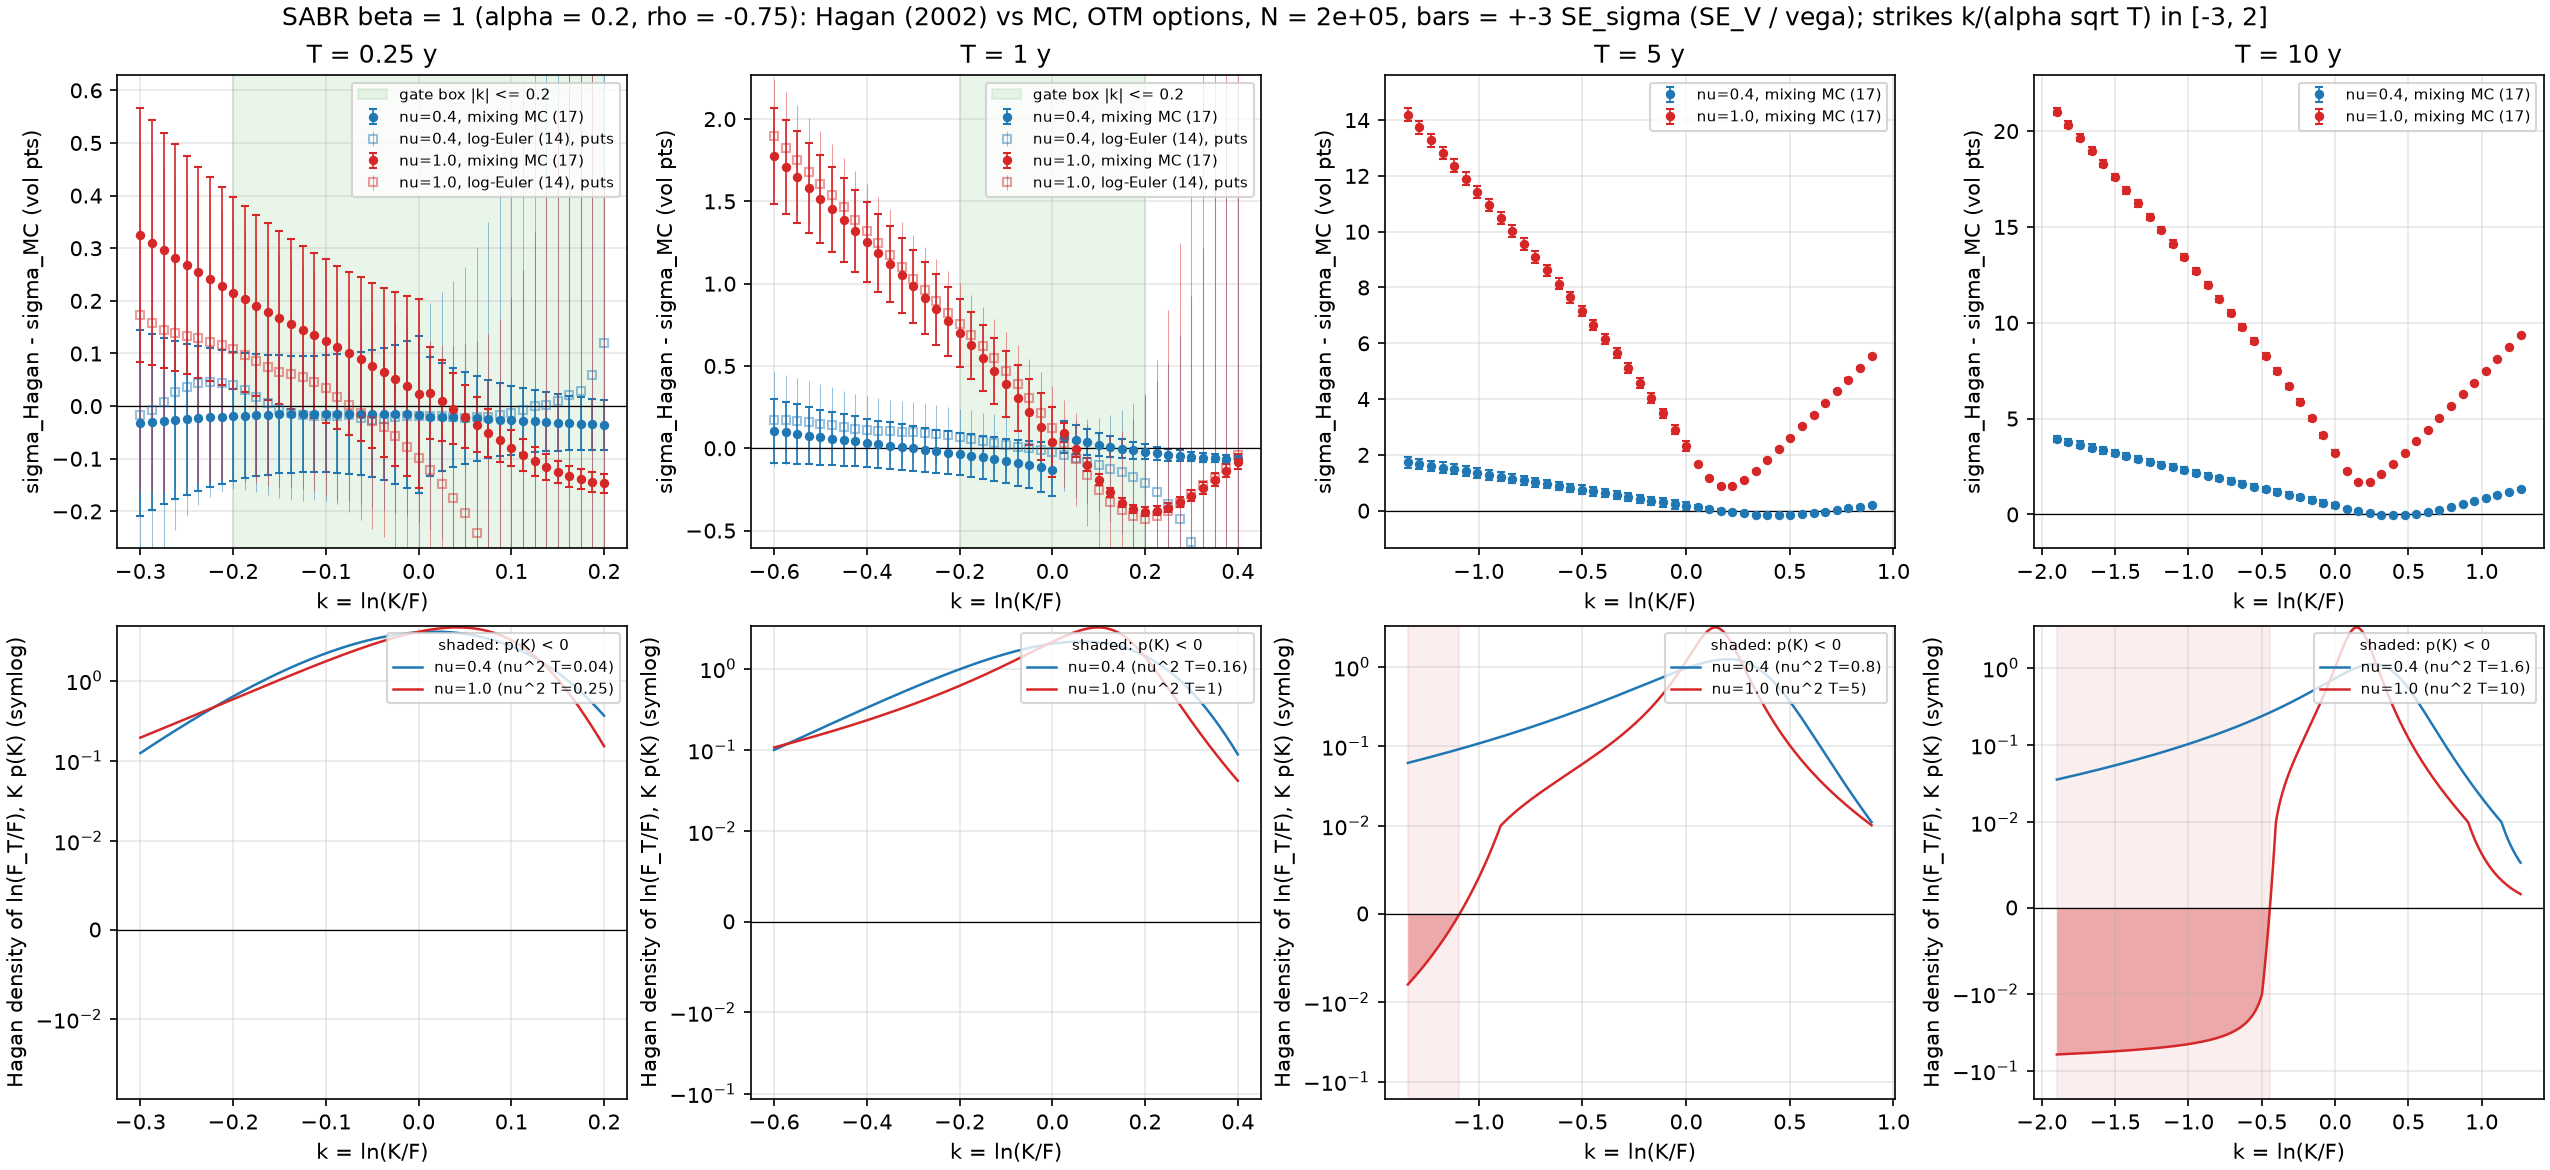
\includegraphics[width=\textwidth]{sabr_hagan_vs_mc.png}
\caption{SABR $\beta=1$ ($\alpha=0.2$, $\rho=-0.75$): Hagan against MC, OTM options, $N=2\times10^5$. Top row:
$\sigma_H-\sigma_{\text{MC}}$ in vol points with bars $\pm3\,\SE_\sigma$, for $\nu=0.4$ (blue) and $\nu=1$ (red), at
$T=0.25,1,5,10$; the green area is the gate box ($|k|\le0.2$). Bottom row: density implied by Hagan's formula
(second differences of Black), with negative-density regions shaded.}
\label{fig:sabr-hagan-mc}
\end{figure}

Figure~\ref{fig:sabr-hagan-mc} compares Hagan with the conditional estimator on strikes
$k/(\alpha\sqrt T)\in[-3,2]$. Table~\ref{tab:sabr-degr} reports, for each panel, the largest error among the points
resolved by the MC ($|z|>3$) and the minimum of the density $K\,p(K)$ implied by Hagan.

\begin{itemize}
\item The error grows with $\nu^2T$ and with $|k|$, and is largest at low strikes: Hagan is too high in the left wing.
\item The density becomes negative only at $\nu=1$ for $T=5$ and $T=10$, at low strikes.
\item Inside the gate box ($T\le1$, $|k|\le0.2$) at $\nu=0.4$ the error stays below the noise; at $\nu=1$ it does
not.
\end{itemize}

\begin{table}[t]
\centering
\small
\caption{Degradation of Hagan's formula ($\alpha=0.2$, $\rho=-0.75$): maximum error among the points resolved by
the MC, and minimum of the implied density.}
\label{tab:sabr-degr}
\begin{tabular*}{\textwidth}{@{\extracolsep{\fill}}rrrlrr@{}}
\toprule
$\nu$ & $T$ & $\nu^2T$ & max error (vol points) & at $k=$ & $\min K\,p(K)$\\
\midrule
0.4 & 0.25 & 0.04 & none resolved ($\max|z|=2.2$) & -- & $+0.12$\\
0.4 & 1 & 0.16 & 0.065 & $+0.40$ & $+0.088$\\
0.4 & 5 & 0.8 & 1.74 & $-1.34$ & $+0.011$\\
0.4 & 10 & 1.6 & 3.94 & $-1.90$ & $+0.0053$\\
1 & 0.25 & 0.25 & 0.33 & $-0.30$ & $+0.15$\\
1 & 1 & 1 & 1.78 & $-0.60$ & $+0.042$\\
1 & 5 & 5 & 14.2 & $-1.34$ & $-0.0080$\\
1 & 10 & 10 & 21.0 & $-1.90$ & $-0.061$\\
\bottomrule
\end{tabular*}
\end{table}

\subsection{\texorpdfstring{The validated domain: $\nu^2T\le0.16$}{The validated domain: ν²T ≤ 0.16}}
The gate holds for set G, that is, for $\nu^2T\le0.16$. An independent check, with a ``true'' model price computed
without the project code, shows that within the \emph{same} box ($T\le1$, $|k|\le0.2$) the gate fails as soon as
$\nu$ is realistic for the SPX:
\begin{itemize}
\item $\alpha=0.18$, $\rho=-0.7$, $\nu=1$, $T=0.5$ ($\nu^2T=0.5$): Hagan is $+0.40$ vol points above the model at
$k=-0.2$, that is, 5.4 SE;
\item $\alpha=0.2$, $\rho=-0.75$, $\nu=1$, $T=1$ ($\nu^2T=1$): $+0.82$ vol points at $k=-0.2$, that is, 10 SE.
\end{itemize}
This is the error of the Hagan expansion, not a code error.

\begin{attenzione}[title={Hagan as a parametrization, not as a model}]
In the SPX calibration (Chapter~\ref{cap:calibrazione}) \emph{every} expiry has $\nu^2T$ between 0.35 and 0.89,
outside the validated domain. The calibrated SABR smiles should therefore be read as \emph{parametrizations} of the
smile through Hagan's formula, not as the SABR dynamics. Pricing an exotic with a SABR MC on the same parameters
would give prices inconsistent with the vanillas used for calibration.
\end{attenzione}

\section{\texorpdfstring{Loss of martingality for $\rho>0$}{Loss of martingality for ρ>0}}
\label{sec:sabr-rho-pos}
For $\rho>0$ and $\beta=1$, $F$ is a \emph{strict} local martingale: $\E F_T<F$. Intuitively, with positive
correlation the volatility explodes precisely when the forward rises, and part of the mass ``escapes to infinity''.

The consequences are subtle.
\begin{itemize}
\item The log-Euler scheme \eqref{eq:sabr-euler} is an \emph{exact} martingale for every $\rho$. For $\rho>0$ its
calls (and those obtained via parity with $F$) target $P_{\text{model}}+\DF(F-K)$, not the model call.
\item The conditional estimator, on the other hand, prices the model call. The two methods of the same function
therefore have different expected values for calls with $\rho>0$; on puts they agree.
\item In the model, call and put implied volatilities at the same strike differ.
\item In practice the sample mean of $\hat F_T$ stays below $F$, because the missing mass lies on paths that are never
sampled: the error shows up as an unreliable SE rather than as a visible bias.
\end{itemize}
\begin{esempio}[title={Example: how large the effect is}]
$\alpha=0.3$, $\rho=+0.5$, $\nu=1$, $T=5$. Two independent methods give
\[
\frac{\E F_T}{F}-1=-0.1668\pm0.0003\qquad\text{and}\qquad{-0.1620}\pm0.0016 .
\]
At $\rho=-0.5$ the same computation gives $0.0000\pm0.0001$.
\end{esempio}

On the SPX $\rho<0$, so parity with $F$ holds. But the rule stands: parity with $F$ is the model's parity \emph{only}
for $\rho\le0$.

\section{Numerical pitfalls}
\begin{enumerate}
\item \textbf{$z/x(z)$ as $z\to0$}: $0/0$. Series for $|z|<10^{-3}$; and since \code{np.where} evaluates both
branches, $z$ is replaced by a dummy value in the direct branch.
\item \textbf{$\rho\to\pm1$}: cancellation in $x(z)$. Branch on sign and bound $|\rho|\le0.999$.
\item \textbf{Non-positive volatility} from $1+c_1T\le0$: \code{NaN} with a warning, never clip.
\item \textbf{Smile with arbitrage} in the wings and at long $T$: do not use the formula as a density source outside
its domain of validity.
\item \textbf{Hagan treated as the truth}: a gate at long $T$ or high $\nu$ fails because of the expansion, not the
code.
\item \textbf{Step bias}: the left-point integrated variance is low by about $\tfrac12\nu^2\Delta$; in the wings the
correlation term also matters. Steps per expiry and a size check.
\item \textbf{Trapezoidal rule only in the drift} of log-Euler: it breaks the martingale property.
\item \textbf{Heavy right tail}: calls with infinite variance for $\rho>-1/\sqrt2$. Simulate puts.
\item \textbf{Positivity}: Euler on $F$ or on $\alpha$ (instead of on their logarithms) can give negative values.
\item \textbf{Gate in volatility space}: inverting a noisy price can fail in the wings. Gate in price space.
\item \textbf{ATM inversion above the ceiling} for $\rho<0$: no root; \code{NaN}, never discard silently.
\end{enumerate}

\needspace{6\baselineskip}
\begin{riassunto}
\begin{itemize}
\item SABR: lognormal volatility correlated with the forward; $\beta=1$ chosen a priori (not identifiable, a choice of
dynamics).
\item Hagan: $\sigma_H=\alpha\,\big(z/x(z)\big)(1+c_1T)$; ``distance'' intuition with speed $D(\nu u)$. Evaluated
with a series, branching on sign, and \code{log1p}.
\item Three knobs: $\alpha$ level, $\rho\nu$ skew, $\nu^2/\alpha$ curvature. $\alpha$ from the ATM volatility by
solving a quadratic; for $\rho<0$ there is a ceiling $b^2/(4|a|)$.
\item MC: exact $\alpha$, log-Euler a martingale of order 1; conditional estimator of order 2. Gate on puts, in price
space, 250 steps at every expiry.
\item The formula holds for small $\nu^2T$: validated domain $\nu^2T\le0.16$. Beyond it, errors of tenths of a vol
point already at $T\le1$, and negative densities at large $\nu^2T$.
\item For $\rho>0$ the forward is not a martingale: parity with $F$ holds only for $\rho\le0$.
\end{itemize}
\end{riassunto}

\needspace{6\baselineskip}
\begin{domande}
\begin{enumerate}
\item Why is $\beta$ not calibrated? What changes if $\beta=1$ is chosen instead of $\beta=0.5$?
\item Explain intuitively why $\rho<0$ gives a negative skew.
\item Why is $2\sigma_{\mathrm{ATM}}/(b+\sqrt{b^2+4a\sigma_{\mathrm{ATM}}})$ used to invert the ATM volatility? When
does no solution exist?
\item Why is ``argument minus 1'' passed to \code{log1p} instead of computing the logarithm directly?
\item Why does the SABR MC compare puts, and why in price space?
\item The log-Euler scheme fails the 3 SE step-halving test: is there a bug? What proves it?
\item Under what conditions does Hagan's formula become unreliable, and how do you notice?
\item What happens to put--call parity with $F$ when $\rho>0$?
\end{enumerate}
\end{domande}
